\chapter{Resultados Preliminares}
Los resultados presentados a continuaci\'{o}n se obtienen mediante trabajo conjunto con David Ricardo Figueroa y Gian Pietro Miscione del grupo COBO de la Universidad de los Andes. Estos resultados fueron obtenidos de manera colaborativa. Estos datos son presentados aqu\'{i} como resultados preliminares ya que no han sido todav\'{i}a publicados y no aparecen en otro documento de tesis. Sin embargo, es importantes para contextualizar los resultados presentados en el cap\'{i}tulo 6\\
\section{Par\'{a}metros de los \'{a}ngulos dihedros de Estafiloxantina}
\subsection*{Par\'{a}metros del grupo \ce{O1-C22-C23-C24}}
El grupo COBO realiz\'{o} las optimizaciones QM mencionadas en la secci\'{o}n \ref{sec:qm}, como en las optimizaciones se obtuvieron valores discretos con m\'{a}ximos y m\'{i}nimos similares, entonces estos valores se ajustaron a una sola funci\'{o}n coseno trasladada en los ejes $X$ y $Y$. En el ajuste se encuentra que el potencial dih\'{e}drico es:
\begin{equation}
    V(\phi)=3.222 \left[1+cos(2\phi-180^{\circ})\right]k\mathrm{cal/mol}.
\end{equation}
Este potencial posee tres m\'{i}nimos locales: En $\phi=-180^{\circ}$,$\phi=180^{\circ}$ y $\phi=0^{\circ}$. Los valores $-180^{\circ}$ y $180^{\circ}$ corresponden a la conformaci\'{o}n \textit{trans}, mientras que $0^{\circ}$ corresponde a una conformaci\'{o}n \textit{cis}. Las dos conformaciones est\'{a}n separadas por barreras con una amplitud del orden de $6k\mathrm{cal/mol}$. Estas barreras son m\'{a}s altas que la energ\'{i}a t\'{e}rmica de una mol de \'{a}tomos a $T=323$K puesto que $E_{k}=N_{A}k_{B}T=641k\mathrm{cal/mol}$. Esto nos indica que la probabilidad de que los dihedros de STX cambien de conformaci\'{o}n es baja, puesto que $p=exp(-E/k_{B}T)/Z\sim10^{-6}/Z$ (con $Z>1$). Esto asegura que la conformaci\'{o}n de la mol\'{e}cula no cambiar\'{a} durante la duraci\'{o}n de las simulaciones, reflejando la alta rigidez del segmento dianeuroesporenoico de estafiloxantina. Adicionalmente, este potencial garantiza una configuraci\'{o}n plana de la mol\'{e}cula.

\subsection*{Par\'{a}metros de la cadena diaponeurosporenoica desde \ce{C23} hasta \ce{C47}}
En la figura \ref{fig:potdih} se encuentra que para el complejo de enlaces dobles conjugados \ce{C=C-C=C}, que va desde \ce{C23} hasta  \ce{C41} el potencial escogido presenta m\'{i}nimos de energ\'{i}a en la conformaci\'{o}n trans, cuyos \'{a}ngulos correspondientes son $\phi=-180^{\circ}$ y $\phi=180^{\circ}$. Otro m\'{i}nimo local aparece en la conformaci\'{o}n \textit{cis}. Sin embargo para alcanzar este m\'{i}nimo se requiere sobrepasar una barrera energ\'{e}tica de alrededor  de $6k\mathrm{cal/mol}$ que de manera similar al caso de \ce{O1-C22-C23-C24}, no es probable de superar. Por lo tanto, el resto de los dihedros de la cadena de diaponeuroesporeno estar\'{a}n en estado trans generando una cadena completamente extendida, planar y r\'{i}gida.\\ 
\begin{figure}[h]
\begin{center}
    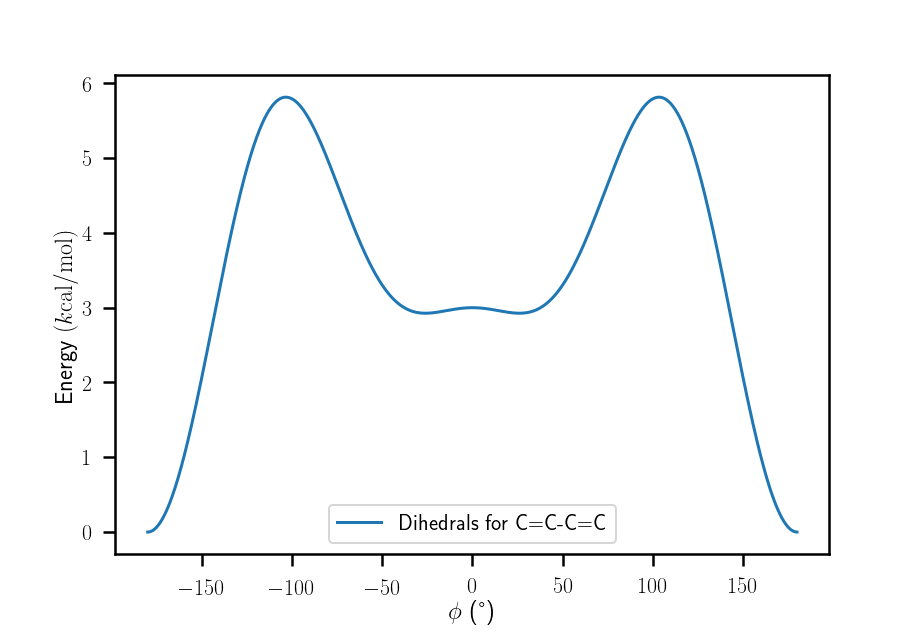
\includegraphics[scale=0.4]{Plots/Dihedrals for C=C-C=C.png}
  \caption{Energ\'{i}a potencial dih\'{e}drica de los enlaces dobles conjugados de la forma \ce{C=C-C=C} en funci\'{o}n del \'{a}ngulo dihedral $\phi$.}
  \label{fig:potdih}
\end{center}
\end{figure}



\section{Orientaci\'{o}n de la Estafiloxantina y Posici\'{o}n de su Az\'{u}car}

Se ha especulado en la literatura con base en la estructura de la mol\'{e}cula que la estafiloxantina probablemente se enuentra en una conformaci\'{o}n vertical debido a que una configuraci\'{o}n horizontal ser\'{i}a dificil de acomodar en la membrana debido a el caracter r\'{i}gido de la cadena diaponeuroesporenica. \cite{Gruszecki2004CarotenoidsProperties}, \cite{Marquardt2016CholesterolsBilayers}, Se ha sugerido que la cadena se mantiene en una orientaci\'{o}n vertical en donde la larga cadena diaponeuroesporenoica abarca las dos monocapas de la membrana.. Con el fin de explorar esta hip\'{o}tesis en las simulaciones, se midi\'{o} la distribuci\'{o}n de orientaciones de estafiloxantina. Se define el \'{a}ngulo de orientaci\'{o}n de STX como el \'{a}ngulo m\'{a}s peque\~{n}o entre el vector normal a la membrana y el vector que recorre la cadena diaponeuresporenoica (o poli\'{e}nica), ver figura \ref{fig:stxangdef}. En la figura puede observarse que el \'{a}ngulo es de 0\textdegree  cuando la cadena de STX se encuentra en una orientaci\'{o}n vertical mientras que el \'{a}ngulo ser\'{a} de 90\textdegree  si  la cadena de STX se encuentra en una orientaci\'{o}n horizontal.\\
%resultados
%#orientaci\'{o}n
\begin{figure}[h]
\begin{center}
  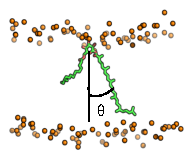
\includegraphics[scale=1.4]{Plots/angle_1stx.pdf}
  \caption{Definici\'{o}n del \'{a}ngulo de orientaci\'{o}n de la estafiloxantina. Se toma el \'{a}ngulo definido por el vector de la cadena diaponeurosporenoica y el vector normal a la membrana. Figura obtenida con Pymol.}
  \label{fig:stxangdef}
\end{center}
\end{figure}
Se obtuvieron distribuciones del \'{a}ngulo de orientaci\'{o}n de STX y estas se graficaron en funci\'{o}n de la distancia relativa entre la posici\'{o}n  del az\'{u}car $z_s$ y la posici\'{o}n de los f\'{o}sforos de la membrana $z_P$. Esta distancia se define como $d=z_s-z_P$ y representan a profunidad de inserci\'{o}n de la cabeza polar de STX. Al graficar la profundidad de inserci\'{o}n versus el angulo de orientaci\'{o}n de STX exploramos si estan correlacionados estos dos par\'{a}metros. Las distribuciones de la orientaci\'{o}n obtenidas tienen la forma de una distribuci\'{o}n normal para una estafiloxantina inmersa en DMPG con tendencia a una orientaci\'{o}n m\'{a}s horizontal, siendo $\langle\theta\rangle=(52\pm13)^{\circ}$ el \'{a}ngulo medio para 15\%STX-DMPG, mientras que para 15\%STX-DPPG: $\langle\theta\rangle=(45\pm14)^{\circ}$. Este resultado sugiere que en DMPG estafiloxantina prefiere mantener  su grupo diaponeuroesporenico con un angulo pronunciado y no una orientaci\'{o}n vertical. En DPPG, se obtiene una distribuci\'{o}n binomial en donde una fracci\'{o}n de las mol\'{e}culas prefiere un angulo pronunciado y otra fracci\'{o}n prefiere una orientaci\'{o}n vertical. Cuando se introduce la estafiloxantina con los nuevos par\'{a}metros ``STX r\'{i}gida'', tiende a desaparecer esta distribuci\'{o}n bimodal para DPPG. Cuando la concentraci\'{o}n es del 15\%, vuelve a aparecer la distribuci\'{o}n bimodal. Esto puede deberse a que al ser DPPG un l\'{i}pido con m\'{a}s carbonos que DMPG, el espesor de la membrana ser\'{a} m\'{a}s largo y como el espesor es mayor, entonces la estafiloxantina podr\'{a} muestrear una mayor cantidad de \'{a}ngulos. El grupo diaponeuroesporenico tiene 30\ce{C} de largo. Una configuraci\'{o}n vertical de la mol\'{e}cula en DMPG proyectar\'{i}a el grupo diaponeuroespor\'{e}nico hasta la interface acuosa de la monocapa inferior, lo cual podr\'{i}a implicar un costo energ\'{e}tico alto. La orientaci\'{o}n horizontal parece no afectar demasiado a los l\'{i}pidos de DMPG vecinos ya que, debido al grado de libertad rotacional de sus cadenas aciles, estas cadenas pueden acomodarse alrededor del grupo diaponeuroespor\'{e}nico sin problema.  Al aumentar el grosor de la membrana, como es el caso de DPPG, es mas probable que se genere una orientaci\'{o}n vertical de la mol\'{e}cula ya que el grupo diaponeuroespor\'{e}nico no alcanzar\'{i}a a proyectarse a la fase acuosa de la monocapa inferior. Para explicar esta hip\'{o}tesis con mas cuidado se podr\'{i}a proponer hacer un barrido por umbrella sampling para estudiar los costos energ\'{e}ticos asociados con la orientaci\'{o}n de la mol\'{e}cula para entender el costo energ\'{e}tico de una orientaci\'{o}n vertical. Es interesante observar que la muestra con 15\% de estafiloxantina muestra una propensidad de orientar las mol\'{e}culas de manera vertical. Al aumentar la concentraci\'{o}n de STX el costo energ\'{e}tico de tener la mol\'{e}cula mas horizontal parece aumentar. \\

% \begin{figure}[h]
% \begin{center}
%   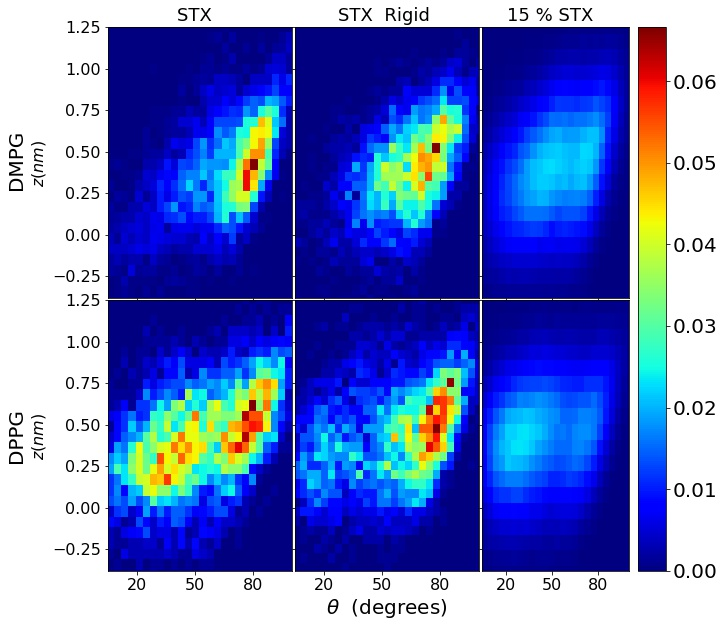
\includegraphics[scale=0.5]{Plots/orientation_vs_z.png}
%   \caption{Orientaci\'{o}n de la estafiloxantina en funci\'{o}n de la coordenada $z$ de inmersi\'{o}n del az\'{u}car. Se toma el \'{a}ngulo definido por el vector de la cadena diaponeurosporenoica y el vector normal a la membrana. Figura obtenida en conjunto con el grupo COBO.}
%   \label{fig:stxangz}
% \end{center}
% \end{figure}

Para un 15\% de STX aparecen los dos picos tanto en el caso DMPG como en el caso DPPG y los rangos posibles son similares, pero la media para el caso de DMPG es mayor que para el caso de DPPG, esto nos indica que el \'{a}ngulo tiende a ser m\'{a}s vertical a un 15\% de STX inmersa en DPPG.\\ 

Por otro lado, en los diagramas de dispersi\'{o}n de la posici\'{o}n del az\'{u}car respecto al \'{a}ngulo de orientaci\'{o}n, se observa una ligera tendencia a la inserci\'{o}n del az\'{u}car dentro de la membrana a medida que aumenta el \'{a}ngulo de orientaci\'{o}n. Esta caracter\'{i}stica desaparece para el caso 15\% STX en DPPG, en donde no se observa una correlaci\'{o}n entre el \'{a}ngulo y la posici\'{o}n del az\'{u}car.\\
\
section{Par\'{a}metro de Orden}
%#par\'{a}metro de orden
%En la figura FIGURA se encuentra el par\'{a}metro de orden de los l\'{i}pidos para todos los sistemas: Figura 
El par\'{a}metro de orden de los l\'{i}pidos se hall\'{o} para cada una de las cadenas:
a): cadena 1 DMPG, b) cadena 2 DMPG, c): cadena 1 DPPG, d) cadena 2 DPPG. El par\'{a}metro de orden de los l\'{i}pidos incrementa significativamente  cuando la membrana contiene 15\% de STX llegando a ser este aumento de entre 0.02 a 0.04 cuando miramos los carbonos C4 a C6 de todos los casos, es decir, los l\'{i}pidos de la membrana est\'{a}n m\'{a}s organizados cuando hay mayor contenido de STX . Adem\'{a}s, si comparamos los casos de DMPG contra DPPG vemos que el par\'{a}metro de orden es menor en el orden de 0.01 entre los carbonos C4 a C6 para el caso DMPG que para el caso DPPG, entonces se puede ver que la membrana est\'{a} m\'{a}s ordenada cuando el 15\% de STX est\'{a} inmerso en DPPG. Otra diferencia se encuentra entre las cadenas 1 y 2 para cada caso. En ambos sistemas la cadena 2 presenta un valle en el \'{a}tomo C2, esto debido a la posici\'{o}n de la cadena con respecto a la cabeza polar.\\

%En la figura FIGURA se muestra 
Para el caso de la estafiloxantina se hall\'{o} el par\'{a}metro de orden para su cadena acil en los sistemas: a): DMPG, b): DPPG, se escogi\'{o} esta cadena ya que al estar compuesta de carbones con enlaces sencillos los grados de libertad de esta cadena acil permite su reorientaci\'{o}n, generando una distribuci\'{o}n adecuada y evitando los artefactos que se esperar\'{i}a observar en la cadena r\'{i}gida del grupo diaponeuroespor\'{e}nico en la medici\'{o}n del par\'{a}metro de orden. Para los casos de una sola STX no hubo un incremento significativo del par\'{a}metro de orden de las cadenas aciles de DMPG y DPPG, pero para un 15\% increment\'{o} significativamente excepto para el primer \'{a}tomo de la cadena acil. \\ 

Ya que el par\'{a}metro de orden est\'{a} relacionado con las constantes el\'{a}sticas del sistema ver Douliez et. al. \cite{Douliez1998OnBiomembranes}, esto significa, de forma cualitativa, que la membrana debe volverse  m\'{a}s r\'{i}gida en presencia de estafiloxantina.\\

\section{Espesor de la Membrana}
%espesor de la membrana

%En la figura \ref{fig:thick},
Mediante la herramienta de gromacs se obtiene la densidad electr\'{o}nica normalizada respecto al eje z de la membrana (normal), las posiciones de los fosfatos se obtienen con los m\'{a}ximos de la densidad electr\'{o}nica en todos los sistemas. Realizando la diferencia entre estos valores, el espesor de la membrana para DMPG es de $3.5n$m, mientras que para DPPG es $3.8n$m. La densidad electr\'{o}nica de la cadena acil de los l\'{i}pidos no es cero en el centro de la membrana, esto quiere decir que hay interdigitaci\'{o}n. El ox\'{i}geno \ce{O3},  presente en el az\'{u}car de STX, est\'{a} m\'{a}s inmerso en la membrana puesto que su posici\'{o}n es menor a la del fosfato de la derecha, esto quiere decir que el az\'{u}car est\'{a} hacia adentro de la membrana. En todos los casos la posici\'{o}n de este \ce{O3}, en promedio, est\'{a} en el mismo lugar. Por otro lado, la densidad electr\'{o}nica es menor para los l\'{i}pidos que para los ox\'{i}genos \ce{O3} de la estafiloxantina.\\
% \begin{figure}[h]
% \begin{center}
%   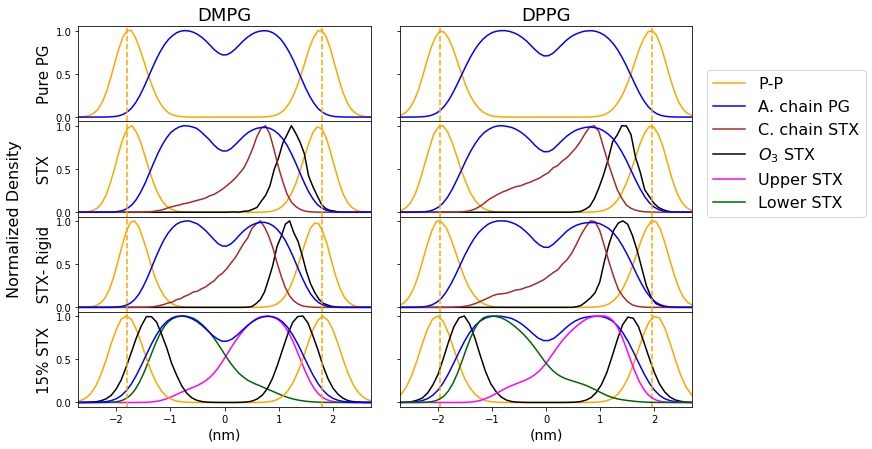
\includegraphics[scale=0.5]{Plots/Thickness_all4x2_nowat.jpg}
%   \caption{Densidad electr\'{o}nica de diferentes \'{a}tomos en la memgrana. En dorado aparecen las densidad de los fosforos, pertenencientes a los l\'{i}pidos. Con los picos se obtiene el espesor de la membrana. }
%   \label{fig:thick}
% \end{center}
% \end{figure}
\section{\'{A}rea global por L\'{i}pido}
Mediante la herramienta de gromacs y la ecuaci\'{o}n \ref{eq:aplglobal} se halla el \'{a}rea global de todas las mol\'{e}culas presentes en la membrana sin distinguir su tipo. Tanto para los sistemas compuestos por DMPG como para los sistemas compuestos por DPPG, se observa una disminuci\'{o}n en los picos (modas) del \'{a}rea por l\'{i}pido al agregar mayores cantidades de estafiloxantina. Por otro lado  las modas, que en la distribuci\'{o}n normal coinciden con los valores medios (mostrados en l\'{i}neas punteadas) disminuyen sus valores, tenemos que las distribuciones se sobrelapan en m\'{a}s del 34\% de las gr\'{a}ficas, tal como se ve en el error est\'{a}ndar mostrado en la figura \ref{fig:aplglobal}, lo cual indica que los cambios registrados no son  significativos. Por otro lado, es importante notar que, en presencia de STX, la distribuci\'{o}n incluye las areas por lipido tanto de los l\'{i}pidos PG y STX. Esto tiene un impacto en como se comporta la distribuci\'{o}n ya que contiene informaci\'{o}n de dos tipos de mol\'{e}culas.\\

\begin{figure}[h]
\begin{center}
  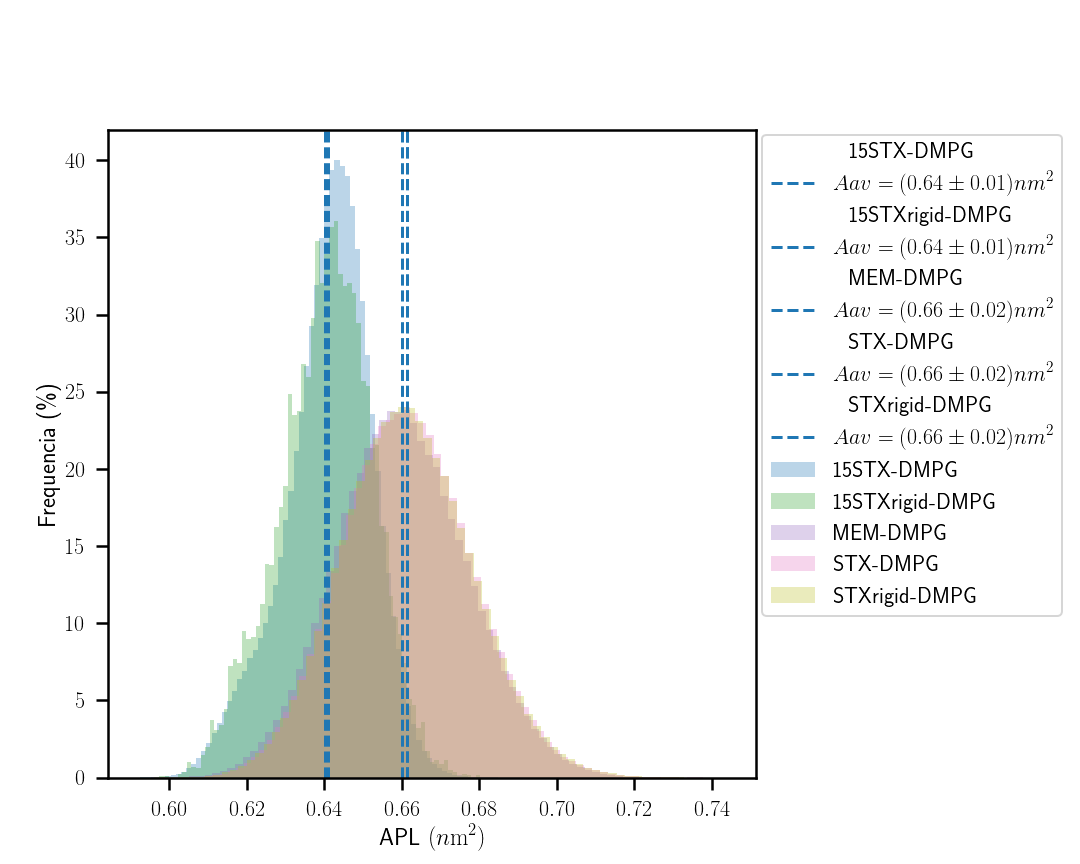
\includegraphics[scale=0.2]{Plots/APL_hist_DMPG.png}
  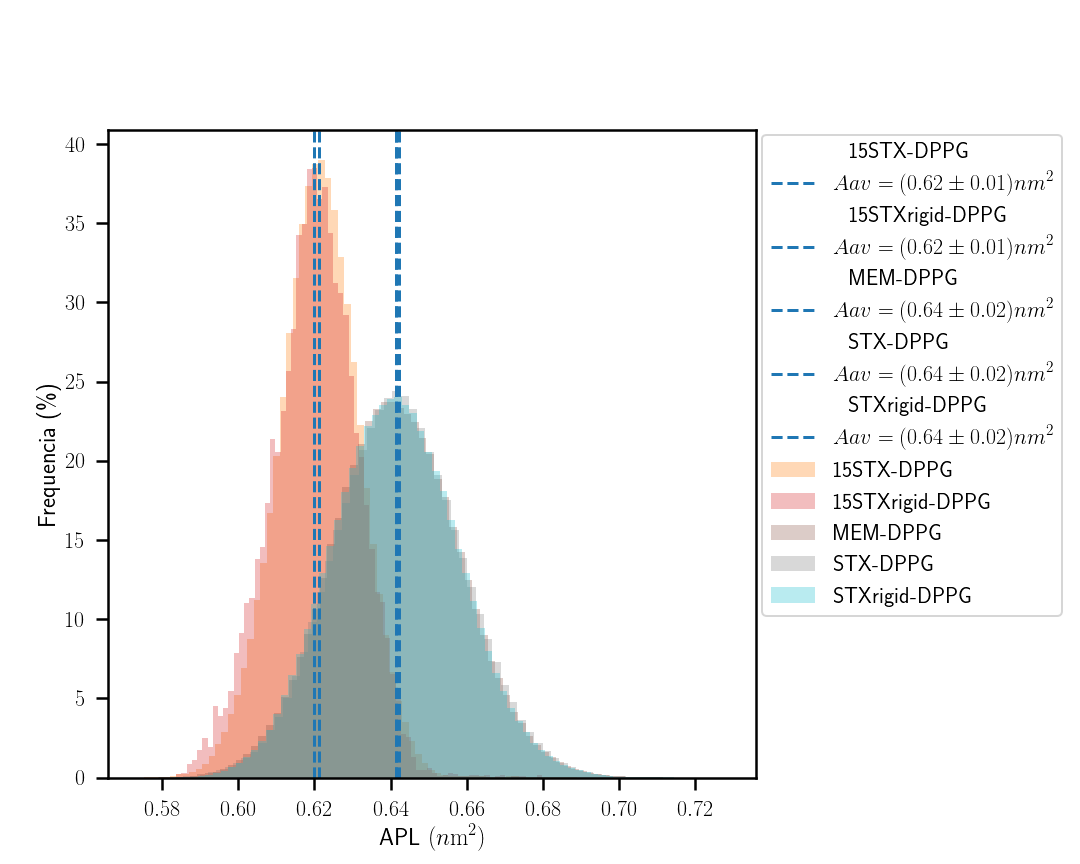
\includegraphics[scale=0.2]{Plots/APL_hist_DPPG.png}
  \caption{\'{A}rea por l\'{i}pido global, para todas las mol\'{e}culas de la membrana sin distinguir, halladas con la herramienta de gromacs.} 
  \label{fig:aplglobal}
\end{center}
\end{figure}
A modo de resumen, los cambios cualitativos observados cuando hay presencia de estafiloxantina o cuando se comparan los sistemas que contienen DMPG con los sistemas que contienen DPPG son:\\
\'{A}ngulo medio: $\theta_{15STX-DMPG}>\theta_{15STX-DPPG}$ \\
Espesor: $d_{DPPG}=d_{15STX-DPPG}>d_{15STX-DMPG}=d_{DMPG}$ \\
\'{A}rea global por l\'{i}pido: $A_{DMPG}=A_{DPPG}=A_{15STX-DMPG}>A_{15STX-DPPG}$ \\
